%!TEX root = series of tubes.tex

\section{The Design Space of Pipes}\tovi{might want to italicize all words that are part of the design space, such as threadable, tree, star, etc}
Our review of prior art indicates the potential benifits of using interior pipes for adding interactivity to 3D printed objects, although no general purpose tools currently exist for this purpose. To guide the design of such tool, we now proivde a deisgn space of the types of pipes that a maker may want to utlize. We have identified four relevant dimensions of pipe design: openings, path constraints, topologies, and inserted media.  We describe the space below.

\begin{figure}[t]
\centering
    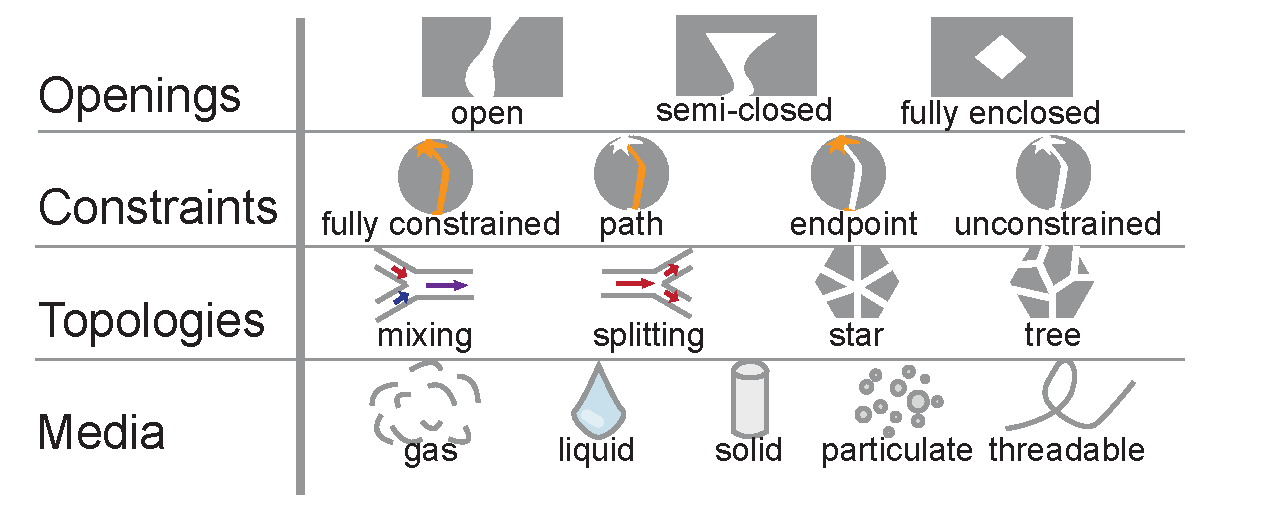
\includegraphics[width=1.0\columnwidth]{figures/tubespace.pdf}
\caption{The design space of pipes.  See text for details. \bjoern{needs full caption.}}
\label{fig:pipespace}
\end{figure}

\subsection{Openings}
Pipes inside solid objects can be either open to the outside on both ends, semi-enclosed, or fully enclosed (see Figure \ref{fig:pipespace}). For interactive devices, openings can be either user-facing (in places a user would for example touch a model); or system-facing, where sensors and actuators may be connected.
%\george{difference between open/return not clear}
%Pipes can have four opening styles: open, return, semi-closed, and fully enclosed .  As we are interested in interactive devices, we distinguish a ``user side"---part of the surface or interior of an object facing its user for interaction; and a ``system side"---where other hardware such as electronics may be connected.  We refer to a pipe which is ``open on the user side'' to have its contents \emph{physically accessible} to a user \emph{at interaction time}.  ``Closed on the user side'' implies physically cut off from the user.  Similarly with the system side.  User or system manipulation of pipe contents are possible even without physical access: e.g., via soundwaves. \george{confusing}

\begin{figure}[t]
\centering
    \includegraphics[width=1.0\columnwidth]{figures/types.png}
\caption{Pipe openings: A shows a pair of open tubes filled with copper paint to power an LED.  B shows a return pipe with EL wire threaded through it.  C shows two semi-closed pipes capped by rubber membranes.  In D, a rabbit has a fully enclosed chamber to modify its weight.}
\label{fig:openings}
\end{figure}

Open pipes may be used to create electronic circuitry.  For example, an open pipe filled with conductive paint and connected to a battery can provide power to an LED (see Figure \ref{fig:openings}A).
%
Semi-enclosed pipes are capped on one side and could be used to create create tactile output. By fabricating a cap from a malleable material and attaching a pump to the open ended, haptic feedback can be generated by raising and depressing the flexible cap (see Figure \ref{fig:openings}C).
%
Fully enclosed pipes (cavities) are entirely internal to the object.  Fully enclosed pipes may be used as weight modifiers~\cite{Prevost-makeitstand} and for object identification~\cite{Willis-infrastructs}, as in Figure \ref{fig:openings}D.  If printed in parts and assembled post-print, enclosed pipes could also contain water or particles that would otherwise fall out.\bjoern{how would you get the particles inside?}\tovi{added this info}

\subsection{Path Constraints}
Depnding on the purpose of the pipe, it's  geometry may be contrainted to sepcific locations within the 3D model. An end-point constrained pipe requires specific start and end points, but the secific route of the internal path is irrelevant. This owuld be the case for circuit schematics, where the electronic compoents have a fixed location, but many routing solutions are valid. In contrast, with a path-constrained pipe it is the shape of the path that is important. For example, threading electroluminescent (EL) wire through a clear pipe enables makers to emulate neon art (see Figure \ref{fig:openings}B). A fully contrained pipe requires both specific terminals as well as a specific path. This would be the case for an interactive  maze (Figure \ref{fig:maze}). Finally, a unconstrained pipe does not need a specific path or terminal points. Using a cavity to modify an object's wieght is an example of an uncontrained pipe.
% Alternatively, the neon sign's output in Figure \ref{fig:neon} is based only on the \emph{path} of the pipe.  Focused on just the exterior features is the touch sensitive toy in Figure \ref{fig:toys}, where pipes must exit the toy at the frontal lobe and parietal lobes to make those \emph{specific locations} touch-sensitive.  A pipe for weight modification does require specific terminals or a specific path (see Figure \ref{fig:openings}D).

\subsection{Pipe Topologies}
Pipe network topologies enable splitting or mixing of media (see Figure \ref{fig:pipespace}).  Star and tree topologies extend the splitting and mixing primitives, encompassing multiple-in and multiple-out configurations; we use star topologies to create different conductive paths in touch-sensitive toys, with a single terminal for swept-frequency capacitive sensing (Figure~\ref{fig:toys}).

\subsection{Media in Pipes}
After printing, different media can be inserted into pipes to change affordances and capabilities. We consider gas, liquids, solids, particulates, and threadables. 
%
Compressible fluids (``gas'') and incompressible fluids (``liquids'')  inside semi-enclosed pipes can create haptic feedback; pressure can also be sensed to act as an input~\cite{Slyper-shape}. Gases can be used as carriers for scents or fog. Conductive liquids like copper paint, when dried, turn pipes into conductive paths and can also fix electronic components in place.
%
%got to here
Filling pipes with solids at print time enables designers to exploit the difference in material properties between pipe and contents. For example, in Printed Optics~\cite{Willis-printedoptics}, different refractive indices between solid cladding material and transparent material inside pipes made light transport along pipes for input and output possible.
%
Particulates, either printed in-place or inserted, can be of varying densities and can contain particles of various and variable size.  A single large particle can be used for display.  Small particles in fluid can provide variable stiffness haptics via jamming \cite{Follmer-jamming}. \bjoern{I thought jamming is about particles in a vacuum? why liquid?}
%
Threadable media, such as regular wire, electroluminescent wire, or commercial fiberoptic cables, can be threaded through pipes post-printing. Threading such media enables addition of conduction, illumination, or optical sensing using materials that can easily be procured, but cannot themselves be printed, e.g., on consumer printers with a single material. 
% This empowers inexpensive printers: for example, a Printed Optics-style interface can be created on a consumer-grade 3D printer with pipes and fiber optic cable.

In the next section we how different pipes within this design space space can be created with the help of our new design tool, \systemname.
